
\section{Identifiant de taille variable}

Certaines structures de données sans résolution de conflits pour séquences
utilisent des identifiants dont la taille est variable à la
génération~\cite{andre2013supporting, preguica2009commutative,
  weiss2009logoot}. Ainsi, les identifiants sont toujours uniques et immuables
une fois générés, mais leur structure contient une liste d'éléments encodant
leur position dans la séquence.  Contrairement aux approches basées sur les
pierres tombales, ces identifiants ne dépendent pas d'autres identifiants afin
d'être intégrés. À ce titre, les suppressions peuvent ne se contentent pas de
masquer les éléments, mais les retirent entièrement de la structure. En
revanche, la liste d'éléments constituants les identifiants est susceptible de
grandir \TODO{impactant les performances}. 

\begin{wrapfigure}{r}{0.5\textwidth}
  \vspace{-32pt} %% (ugly)
  \begin{minipage}[t]{0.5\textwidth}
    \begin{algorithm}[H]
      
\footnotesize
\algrenewcommand{\algorithmiccomment}[1]{\hskip2em$\rhd$ #1}

\newcommand{\comment}[1]{$\rhd$ #1}


\algblockdefx[initially]{initially}{endInitially}
[0] {\textbf{INITIALLY:}} 

\algblockdefx[local]{local}{endLocal}
[0] {\textbf{LOCAL UPDATE:}}

\algsetblockdefx[received]{received}{endReceived}
{65535}{}
[0] {\textbf{RECEIVED UPDATE:}}

\algblockdefx[onInsert]{onLocal}{endOnLocal}
[0] {\textbf{on} insert ($\DARKBLUE{p \in \mathcal{I}},\,\alpha \in \mathcal{A},\,
  \DARKBLUE{q\in\mathcal{I}}$):}
[0] {\textbf{on} delete ($i \in \mathcal{I}$):} 

\algblockdefx[onRemote]{onRemote}{endOnRemote}
[0] {\textbf{on} insert ($i\in\mathcal{I}$):\hfill\comment{once per identifier}}
[0] {\textbf{on} delete ($i\in\mathcal{I}$):\hfill\comment{$i$ has been integrated}}

\newcommand{\LINEFOR}[2]{%
  \algorithmicfor\ {#1}\ \algorithmicdo\ {#2} %
}

\newcommand{\LINEIFTHEN}[2]{%
  \algorithmicif\ {#1}\ \algorithmicthen\ {#2} %
}

\newcommand{\INDSTATE}[1][1]{\State\hspace{\algorithmicindent}}

\begin{algorithmic}[1]
  \Statex
  \initially
    \State $\mathcal{T} \leftarrow \varnothing$; \hfill \comment{the CRDT}
  \endInitially
  
  \local
    \onLocal
    \State \textbf{let} $path \leftarrow \DARKBLUE{\textsc{allocPath}(p.P,\,q.P)}$; \label{line:allocpath}
    \State \textbf{let} $dis \leftarrow \textsc{allocDis}(p,\, path,\, q)$; \label{line:allocdes}
    \State $\textsc{broadcast}('insert',\, \langle path,\, \alpha,\, dis \rangle)$;
    \endOnLocal
    \INDSTATE $\textsc{broadcast}('delete',\,i)$;
  \endLocal
  
  \received
    \onRemote
    \State $\mathcal{T} \leftarrow \mathcal{T} \cup i$;
    \endOnRemote
    \INDSTATE $\mathcal{T} \leftarrow \mathcal{T}\, \backslash\, i$; 
  
\end{algorithmic}

      \caption{\label{repl:algo:crdtabstract} Squelette.}
    \end{algorithm}
  \end{minipage}
  \vspace{-32pt}
\end{wrapfigure}

\TODO{Definir le modèle.}

L'algorithme~\ref{repl:algo:crdtabstract} présente le squelette de cette famille
de structure pour séquence.  Il est divisé en deux parties qui correspondent à
l'exécution locale et l'exécution distante de la réplication
optimiste. Celles-ci sont elles-mêmes divisées en deux types d'évènements
correspondant aux opérations d'insertions et de suppression d'un
élément. L'algorithme met en lumière trois points :

\begin{itemize}
\item [\textbf{signature :}] les opérations sur la séquence répliquée prennent
  pour arguments les identifiants adjacents à l'insertion, au lieu d'un indice
  dans la séquence pour les séquences \TODO{classiques}.
\end{itemize}

\begin{itemize}
\item [\textbf{complexité locale :}] la complexité de l'algorithme est répartie
  entre la génération d'un identifiant locale et son intégration à la structure
  en partie distante.
\item [\textbf{allocation de chemin} :] la taille des identifiants dépend
  principalement de l'allocation d'un chemin dans l'arbre
  (cf. ligne~\ref{line:allocpath}) auquel est ajouté un désambiguateur
  (cf. ligne~\ref{line:allocdes}) afin de garantir l'unicité de l'identifiant.
\end{itemize}

\begin{figure*}
  \centering
  \subfloat[Allocation quasi-optimale]
  [\label{fig:lseq:allocpathexampleA}Cas d'une allocation quasi-optimale]
  {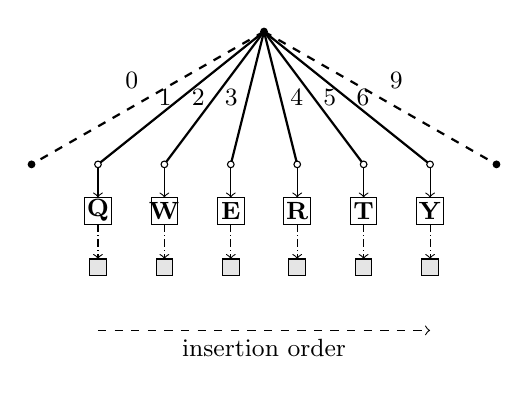
\begin{tikzpicture}[scale=1.2]

  %% node to node
  \small
  \draw[dashed, thick] (0pt,0pt) -- node[anchor=south east]{0} (-70pt,-40pt);
  \draw[thick] (0pt,0pt) -- node[anchor=east]{\DARKBLUE{1}} (-50pt,-40pt);
  \draw[thick] (0pt,0pt) -- node[anchor=east]{\DARKBLUE{2}} (-30pt,-40pt);
  \draw[thick] (0pt,0pt) -- node[anchor=east]{\DARKBLUE{3}} (-10pt,-40pt);
  \draw[thick] (0pt,0pt) -- node[anchor=west]{\DARKBLUE{4}} ( 10pt,-40pt);
  \draw[thick] (0pt,0pt) -- node[anchor=west]{\DARKBLUE{5}} ( 30pt,-40pt);
  \draw[thick] (0pt,0pt) -- node[anchor=west]{\DARKBLUE{6}} ( 50pt,-40pt);
  \draw[dashed, thick] (0pt,0pt) -- node[anchor=south west]{9} ( 70pt,-40pt);

  %% node to element
  \draw[->] (-50pt,-40pt) -- (-50pt,-50pt);
  \draw[->] (-30pt,-40pt) -- (-30pt,-50pt);
  \draw[->] (-10pt,-40pt) -- (-10pt,-50pt);
  \draw[->] ( 10pt,-40pt) -- ( 10pt,-50pt);
  \draw[->] ( 30pt,-40pt) -- ( 30pt,-50pt);
  \draw[->] ( 50pt,-40pt) -- ( 50pt,-50pt);

  %% element to desambiguator
  \draw[->,densely dashdotted] ( -50pt,-58pt) -- ( -50pt,-68.5pt);
  \draw[->,densely dashdotted] ( -30pt,-58pt) -- ( -30pt,-68.5pt);
  \draw[->,densely dashdotted] ( -10pt,-58pt) -- ( -10pt,-68.5pt);
  \draw[->,densely dashdotted] (  10pt,-58pt) -- (  10pt,-68.5pt);
  \draw[->,densely dashdotted] (  30pt,-58pt) -- (  30pt,-68.5pt);
  \draw[->,densely dashdotted] (  50pt,-58pt) -- (  50pt,-68.5pt);

  \draw[fill=black] (  0pt,  0pt) circle (1pt);
  \draw[fill=black] (-70pt,-40pt) circle (1pt);
  \draw[fill=white] (-50pt,-40pt) circle (1pt);
  \draw[fill=white] (-30pt,-40pt) circle (1pt);
  \draw[fill=white] (-10pt,-40pt) circle (1pt);
  \draw[fill=white] ( 10pt,-40pt) circle (1pt);
  \draw[fill=white] ( 30pt,-40pt) circle (1pt);
  \draw[fill=white] ( 50pt,-40pt) circle (1pt);
  \draw[fill=black] ( 70pt,-40pt) circle (1pt);

  %% elements
  \draw[fill=white](-50pt,-54pt)
  node{\textbf{Q}}+(-4pt,-4pt)rectangle+(4pt,4pt) ;
  \draw[fill=white](50pt,-54pt)
  node{\textbf{Y}} +(-4pt,-4pt) rectangle +(4pt,4pt) ;
  \draw[fill=white]( 10pt,-54pt)
  node{\textbf{R}} +(-4pt,-4pt) rectangle +(4pt,4pt) ;
  \draw[fill=white] ( -30pt,-54pt)
  node{\textbf{W}} +(-4pt,-4pt) rectangle +(4pt,4pt) ;
  \draw[fill=white] ( -10pt,-54pt)
  node{\textbf{E}} +(-4pt,-4pt) rectangle +(4pt,4pt) ;
  \draw[fill=white]( 30pt,-54pt)
  node{\textbf{T}} +(-4pt,-4pt) rectangle +(4pt,4pt) ;

  %% desambiguator
  \draw[fill=gray!20] (-50pt,-71pt) +(-2.5pt,-2.5pt) rectangle +(2.5pt,2.5pt);
  \draw[fill=gray!20] (-30pt,-71pt) +(-2.5pt,-2.5pt) rectangle +(2.5pt,2.5pt);
  \draw[fill=gray!20] (-10pt,-71pt) +(-2.5pt,-2.5pt) rectangle +(2.5pt,2.5pt);
  \draw[fill=gray!20] ( 10pt,-71pt) +(-2.5pt,-2.5pt) rectangle +(2.5pt,2.5pt);
  \draw[fill=gray!20] ( 30pt,-71pt) +(-2.5pt,-2.5pt) rectangle +(2.5pt,2.5pt);
  \draw[fill=gray!20] ( 50pt,-71pt) +(-2.5pt,-2.5pt) rectangle +(2.5pt,2.5pt);

  %% insertion order
  \draw[->,dashed] (-50pt, -90pt) -- node[anchor=north]{insertion order}
  (50pt, -90pt);

\end{tikzpicture}
}
  \hspace{40pt}
  \subfloat[Pire cas d'allocation]
  [Pire cas d'allocation]
  {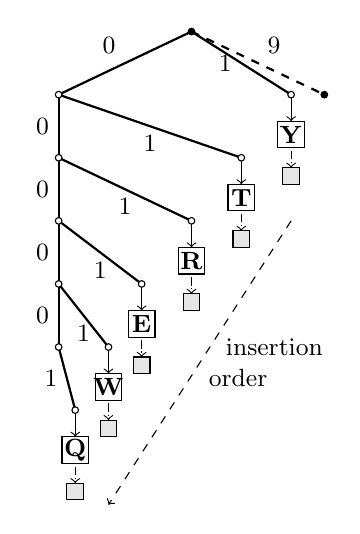
\begin{tikzpicture}[scale=1.2]

\newcommand\Y{-19}
\newcommand\ADDY{-8}

  %% node to node
  \small
  \draw[thick] (0pt,0pt) -- node[anchor=south east]{\DARKBLUE{0}} (-40pt,\Y pt);
  \draw[thick] (0pt,0pt) -- node[anchor=east]{1} (30pt, \Y pt); %% Y
  \draw[thick] (-40pt, \Y pt) -- node[anchor=north]{1} (15pt, 2 * \Y pt); %% T
  \draw[thick] (-40pt, \Y pt) -- node[anchor=east]{\DARKBLUE{0}} (-40pt, 2 * \Y pt); %% 0
  \draw[thick] (-40pt, 2*\Y pt) -- node[anchor=north]{1} (0pt, 3 * \Y pt); %% R
  \draw[thick] (-40pt, 2*\Y pt)-- node[anchor=east]{\DARKBLUE{0}}(-40pt, 3 * \Y pt); %% 0
  \draw[thick] (-40pt, 3*\Y pt) -- node[anchor=north]{1}(-15pt,4 * \Y pt); %% E
  \draw[thick] (-40pt, 3*\Y pt) -- node[anchor=east]{\DARKBLUE{0}}(-40pt,4 * \Y pt); %% 0
  \draw[thick] (-40pt, 4*\Y pt) -- node[anchor=north]{1}(-25pt,5 * \Y pt); %% W
  \draw[thick] (-40pt, 4*\Y pt) -- node[anchor=east]{\DARKBLUE{0}}(-40pt,5 * \Y pt); %% 0
  \draw[thick] (-40pt, 5*\Y pt) -- node[anchor=east]{\DARKBLUE{1}}(-35pt,6 * \Y pt); %% Q

  \draw[dashed, thick] (0pt,0pt) -- node[anchor=south west]{9} (40pt,\Y pt);

  %% node to element
  \draw[->] ( 30pt, \Y pt) -- ( 30pt, \ADDY + \Y pt); %% Y
  \draw[->] ( 15pt, 2* \Y pt) -- ( 15pt, \ADDY + 2 *\Y pt); %% T
  \draw[->] (  0pt, 3 *\Y pt) -- (  0pt, \ADDY + 3 *\Y pt); %% R
  \draw[->] (-15pt, 4 *\Y pt) -- ( -15pt, \ADDY + 4 *\Y pt); %% E
  \draw[->] (-25pt, 5 *\Y pt) -- ( -25pt, \ADDY + 5 *\Y pt); %% W
  \draw[->] (-35pt, 6 *\Y pt) -- ( -35pt, \ADDY + 6 *\Y pt); %% Q

  %% element to desambiguator
  \draw[->,densely dashdotted]
  ( 30pt, \ADDY + \Y pt) -- ( 30pt,2.75*\ADDY+\Y pt); %% Y
  \draw[->,densely dashdotted]
  ( 15pt, \ADDY + 2* \Y pt) -- ( 15pt,2.75*\ADDY+ 2* \Y pt); %% T
  \draw[->,densely dashdotted]
  ( 0pt, \ADDY + 3* \Y pt) -- (  0pt,2.75*\ADDY+ 3* \Y pt); %% R
  \draw[->,densely dashdotted]
  ( -15pt, \ADDY + 4 *\Y pt) -- ( -15pt,2.75*\ADDY+ 4* \Y pt); %% E
  \draw[->,densely dashdotted]
  ( -25pt, \ADDY + 5 *\Y pt) -- ( -25pt,2.75*\ADDY+ 5*\Y pt); %% W
  \draw[->,densely dashdotted]
  ( -35pt, \ADDY + 6* \Y pt) -- ( -35pt,2.75*\ADDY+ 6*\Y pt); %% Q

  %% node
  \draw[fill=black] (0pt,0pt) circle (1pt); %% rooot
  \draw[fill=white] ( 30pt, \Y pt) circle (1pt); %% Y
  \draw[fill=white] (-40pt, \Y pt) circle (1pt); %% 0
  \draw[fill=white] ( 15 pt, 2 * \Y pt) circle (1pt); %% T
  \draw[fill=white] (-40pt, 2 * \Y pt) circle (1pt); %% 0
  \draw[fill=white] (  0 pt, 3 * \Y pt) circle (1pt); %% R
  \draw[fill=white] (-40pt, 3 * \Y pt) circle (1pt); %% 0
  \draw[fill=white] (-15 pt, 4 * \Y pt) circle (1pt); %% E
  \draw[fill=white] (-40pt, 4 * \Y pt) circle (1pt); %% 0
  \draw[fill=white] (-25 pt, 5 * \Y pt) circle (1pt); %% W
  \draw[fill=white] (-40pt, 5 * \Y pt) circle (1pt); %% 0
  \draw[fill=white] (-35 pt, 6 * \Y pt) circle (1pt); %% Q

  \draw[fill=black] ( 40pt, \Y pt) circle (1pt);


  %% elements
  \draw[fill=white] ( 30pt, -4 + \ADDY + \Y pt)
  node{\textbf{Y}} +(-4pt,-4pt) rectangle +(4pt,4pt) ; %% Y
  \draw[fill=white] ( 15pt, -4 + \ADDY +  2 *\Y pt)
  node{\textbf{T}} +(-4pt,-4pt) rectangle +(4pt,4pt) ; %% T
  \draw[fill=white] (  0pt, -4 + \ADDY +  3* \Y pt)
  node{\textbf{R}} +(-4pt,-4pt) rectangle +(4pt,4pt) ; %% R
  \draw[fill=white] (-15pt, -4 + \ADDY + 4 *\Y pt)
  node{\textbf{E}} +(-4pt,-4pt) rectangle +(4pt,4pt) ; %% E
  \draw[fill=white] (-25pt, -4 + \ADDY + 5 * \Y pt)
  node{\textbf{W}} +(-4pt,-4pt) rectangle +(4pt,4pt) ; %% W
  \draw[fill=white] (-35pt, -4 + \ADDY + 6 *\Y pt)
  node{\textbf{Q}} +(-4pt,-4pt) rectangle +(4pt,4pt) ; %% Q

  %% desambiguator
  \draw[fill=gray!20]( 30pt, -2.5 + 2.75 * \ADDY + \Y pt)
  +(-2.5pt,-2.5pt) rectangle +(2.5pt,2.5pt);
  \draw[fill=gray!20]( 15pt, -2.5 + 2.75 * \ADDY +2 *\Y pt)
  +(-2.5pt,-2.5pt) rectangle +(2.5pt,2.5pt);
  \draw[fill=gray!20](  0pt, -2.5 + 2.75 * \ADDY + 3*\Y pt)
  +(-2.5pt,-2.5pt) rectangle +(2.5pt,2.5pt);
  \draw[fill=gray!20](-15pt, -2.5 + 2.75 * \ADDY +4*\Y pt )
  +(-2.5pt,-2.5pt) rectangle +(2.5pt,2.5pt);
  \draw[fill=gray!20](-25pt, -2.5 + 2.75 * \ADDY + 5*\Y pt)
  +(-2.5pt,-2.5pt) rectangle +(2.5pt,2.5pt);
  \draw[fill=gray!20](-35pt, -2.5 + 2.75 * \ADDY +6*\Y pt) 
  +(-2.5pt,-2.5pt) rectangle +(2.5pt,2.5pt);

  %% insertion order
  \draw[->,dashed] (30pt, 3 * \Y pt) -- node[anchor=west,align=left]
  {\ \ insertion\\ order} (-25pt, 7.5 * \Y pt);

\end{tikzpicture}
}
  \caption{\label{fig:lseq:allocpathexample} Deux arbres remplis d'identifiants
    résultant de deux séquences d'édition différentes et dont la séquence finale
    est identique : $QWERTY$. L'allocation des identifiants se fait selon le
    même algorithme qui alloue la branche la plus à gauche de l'arbre. L'arbre
    quasiment optimal ne possède que des branches de profondeur 1 tandis que
    l'arbre pire cas atteint une profondeur de 6.}
\end{figure*}

La figure~\ref{fig:lseq:allocpathexample} illustre les difficultés rencontrées lors
de l'allocation d'identifiants. La figure représente la structure d'arbre
permettant de représenter deux séquences utilisant la fonction d'allocation
suivante : la branche la plus à gauche et la plus petite profondeur de l'arbre
possible. Dans les deux cas, la séquence finale est QWERTY. Toutefois, les
lettres ne sont pas insérées dans un ordre identique. Dans le premier cas, Q est
inséré à l'index 0, suivit de W à l'index 1, suivit de E à l'index 2 etc. Cette
séquence d'opérations d'insertions $[(Q,\,0)$, $(W,\,1)$, $(E,\,2)$\ldots$]$ est
nommée \emph{séquence d'édition}. Dans le second cas, la lettre Y est inséré à
l'index 0, suivit du T à l'index 0 qui va décaler le Y en index 1, etc. La
séquence d'édition qui correspond à ce cas est : $[(Y,\,0)$, $(T,\,0)$,
$(R,\,0)$\ldots$]$.
\begin{itemize}
\item [\textbf{premier cas :}] la fonction $allocPath$ alloue la branche la plus
  à gauche possible. Par conséquent, la séquence d'édition $[(Q,\,0)$,
  $(W,\,1)$, $(E,\,2)$\ldots$]$ conduit aux chemins suivant
  $\langle [1],\,Q\rangle$, $\langle [2],\, W \rangle$,
  $\langle [3],\, E\rangle$, etc. Dans ce cas, la profondeur de l'arbre
  n'augmente jamais. À cet égard, la fonction $allocPath$ est très efficace.
\item [\textbf{second cas :}] la séquence d'édition $[(Y,\,0)$, $(T,\,0)$,
  $(R,\,0)$\ldots$]$ implique une augmentation de la profondeur de l'arbre à
  chaque nouvelle insertion d'élément. En effet, le chemin est choisit est
  toujours celui qui est le petit possible. Les éléments suivant ne bénéficie
  pas de suffisamment de place à la profondeur courante de l'arbre, d'où la
  nécessité d'augmenter sa profondeur. Les chemins en résultant sont :
  $\langle [1],\, Y\rangle$, $\langle[0.1],\,T\rangle$,
  $\langle[0.0.1],\, R\rangle$, etc. La taille des chemins alloués augmente très
  rapidement.
\end{itemize}

Cet exemple montre à quel point l'ordre d'insertion des éléments affecte la
longueur des chemins alloués. Malheureusement, ni l'ordre d'insertion des
éléments, ni la taille finale de la séquence ne peuvent être prédits avec
exactitude. C'est pourquoi les travaux précédents font souvent l'hypothèse d'un
comportement d'édition de gauche-à-droite basés sur observations. Toutefois, il
existe des documents écrit par l'homme dont le comportement ne correspond pas à
celui-ci.

\begin{itemize}
\item [\textbf{Logoot~\cite{weiss2009logoot, weiss2010logootundo} :}]
\item [\textbf{Logoot split~\cite{mehdi2014merging} :}]
\item [\textbf{Treedoc~\cite{shapiro2011comprehensive} :}]
\end{itemize}


%%% Local Variables:
%%% mode: latex
%%% TeX-master: "../../paper"
%%% End:
